\section{Schreibweisen}

\subsection{Fischer Projektion}
\label{sec:fischer}
\begin{itemize}
    \item längste C-Kette von oben nach unten
    \item höchst oxidiertes C-Atom nach oben
    \item letzte anomere C-Atom beschreibt rechts- (D) oder links- (L) drehend: \\
        Wenn OH Gruppe rechts ist, ist es D\\
        Wenn OH Gruppe links ist, ist es L
\end{itemize}

Dabei ist zu beachten, dass durch die Fischerprojektion Enantiomere und Diastomere erfasst werden können. 
Wenn bei dem folgenden Stoff die letzte OH-Gruppe auf der linken Seite wäre, wäre dies ein Diastomer zu dem Stoff. 
Wären alle asymmetrischen C-Atome gespiegelt wäre es ein Enantiomer. \\
$\alpha$-D-Glucose:

%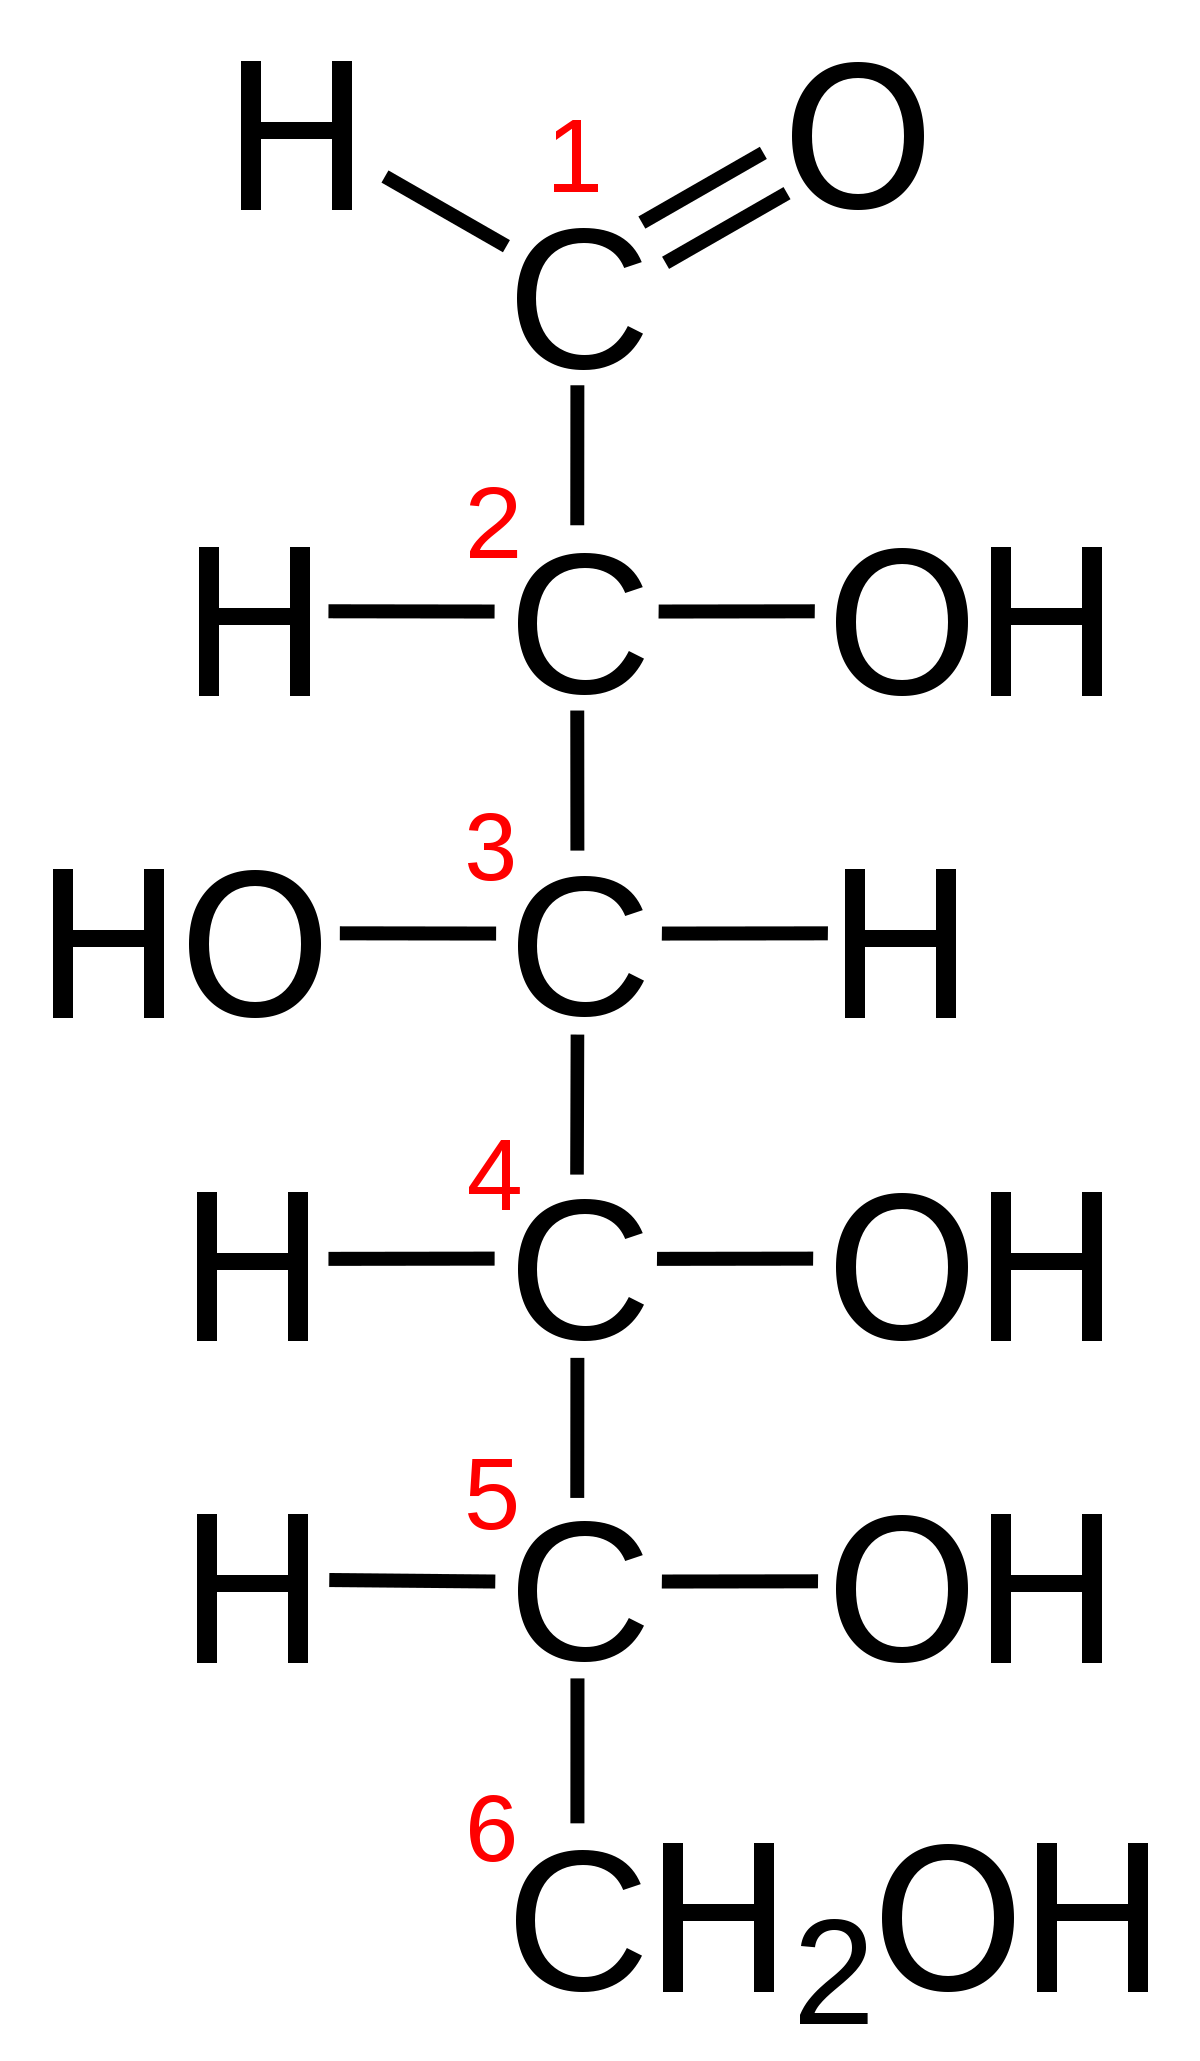
\includegraphics[scale=0.06]{media/naturstoffe/fischer.png}
\scalebox{0.8}{
\chemfig{
    C(-[3]H)(=[1]O)
    -[6]C(-[8]OH)(-[4]H)
    -[6]C(-[4]HO)(-[8]H)
    -[6]C(-[8]OH)(-[4]H)
    -[6]C(-[8]OH)(-[4]H)(-[6]CH_2OH)
}
}

\subsection{Haworth Projektion}
\label{sec:haworth}
D-Glucose:

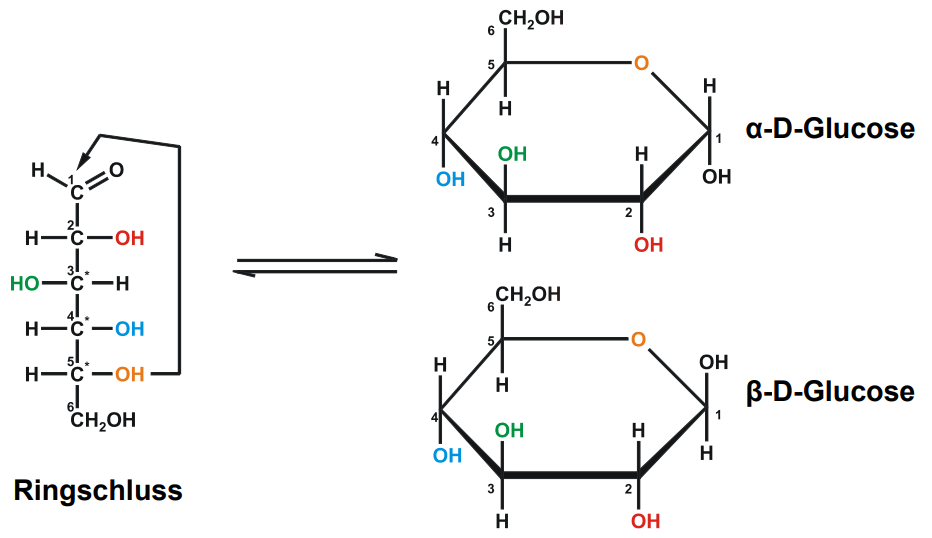
\includegraphics[scale=0.86]{media/naturstoffe/haworth.png}

